\chapter{Conclusion}
\label{chap:conclusion}

\epigraph{\foreignlanguage{USenglish}{Can we actually "know" the
    universe? My God, it's hard enough finding your way around in
    Chinatown.}}{Woody Allen\\\emph{My Philosophy}}
\clearpage

\section{Conclusion}
\subsection{Bilan\ldots}

\lettrine[lines=2, lraise=0.1, nindent=0em, slope=-.5em]%
{L}{es} travaux présentés dans ce manuscrit de thèse ont pour but
d'améliorer les algorithmes de génération et d'exécution de mouvements
pour les robots humanoïdes. Le premier travail présenté a traité de
l'amélioration de la représentation des problèmes d'optimisation afin
de faciliter le prototypage et l'écriture de solveurs, tout en
assurant un haut niveau de sécurité. Un solveur ne doit accepter que
des problèmes qui lui sont adaptés. Une boîte à outils de fonctions de
coût et de contraintes pour l'optimisation de trajectoires a également
été conçue. L'effort théorique principal a été de chercher une
interface telle que la théorie de l'optimisation numérique se trouve
exprimée dans sa totalité tout en excluant les problèmes mal construits
et en maitrisant le coût algorithmique de la résolution des
problèmes. Par exemple, certains gradients ou hessiens peuvent ne pas
être utilisés, mais aucune approximation par différence finie ne peut
être réalisée automatiquement. C'est à l'utilisateur d'explicitement
instancier ce comportement, et d'assumer le coût de calcul
supplémentaire généré par ce type d'approche. Un tel outil est adapté
au post-traitement de trajectoires générées par des algorithmes
aléatoires notamment.

\smallskip

Le second chapitre détaille comment générer une trajectoire de marche
équilibrée sur un sol plan. Les trajectoires sont modélisées sous
forme de tâches et ces dernières sont insérées dans un solveur
temps-réel générant la commande. Le tout forme un contrôleur
polyvalent permettant, entre autres, l'exécution de trajectoires de
marche. Dans des travaux précédents, cette stratégie a déjà été
appliquée pour permettre à un robot humanoïde de marcher mais jusqu'à
présent ces tâches fonctionnaient en boucle ouverte et étaient donc
soumises à une dérive empêchant la réalisation de trajectoires longues
ou nécessitant une grande précision. L'altération du schéma de
contrôle par l'utilisation d'un composant de localisation estimant
cette dérive a permis la réalisation de mouvements d'une grande
précision. La localisation est ici prise en charge par un système de
capture de mouvements.

\smallskip

Cela nous a naturellement amenés à nous poser deux questions abordées
dans le troisième chapitre: peut-on obtenir le même résultat en
utilisant les capteurs embarqués? Peut-on représenter de manière
générique, au-delà de la simple locomotion, des trajectoires
asservies? À la première question, la réponse est, oui, il est
possible de se localiser grâce aux caméras embarquées, mais au prix
d'une précision moindre. Si cette qualité moindre ne gêne pas la
navigation en soi, elle empêche malheureusement toute manipulation
complexe une fois la trajectoire terminée. Il est donc nécessaire de
non seulement asservir la locomotion, mais également la manipulation. La
locomotion nécessite un système de localisation sans dérive, proche
des besoins d'un robot mobile alors que la manipulation nécessite avant
tout un système de localisation dont l'erreur tend vers zéro lors de
la réalisation d'un contact. Un asservissement visuel par exemple est
tout à fait adapté à cet objectif, car plus le robot s'approche de
l'objet, plus la précision croît. Malheureusement, il n'a pas été
possible de tenter une expérimentation intégrant à la fois vision
embarquée, asservissement visuel sur un objet et correction combinée
des trajectoires de locomotion et de manipulation.

\smallskip

Le dernier chapitre, quant à lui, détaille le fonctionnement de
l'architecture robotique mise en place durant cette thèse et qui a été
largement partagée avec d'autres doctorants du groupe. Il est
nécessaire de comprendre le pas franchis puisque l'on est passé d'une
architecture réalisant, soit une lecture des trajectoires articulaires
en boucle ouverte, soit la réalisation d'une pile de tâches avec un
asservissement \emph{ad hoc} dédié au scénario et difficile à
généraliser vers un système fondé sur un ensemble de composants
robotiques réutilisables. S'il n'y a pas eu écriture des composants
robotique, un travail de conception de l'architecture a été nécessaire
afin de permettre l'utilisation conjointe de toutes les capacités du
robot.



\subsection{\ldots et perspectives}


Dans le cadre du travail réalisé pour la modélisation générique des
problèmes d'optimisation, il reste encore de nombreux travaux à mener
dans trois directions différentes. La première est la représentation
informatique de fonctions mathématiques afin d'étendre l'expressivité
des fonctions. L'écriture de fonctions dépendant de plus d'une
variable se trouve compliquée par la nécessité de pouvoir calculer les
gradients combinés issus de la dérivation de plusieurs variables
différentes. La représentation d'espaces mathématiques spécifiques tel
que le groupe spécial Euclidien $\text{SE}(n)$ imposant des
contraintes tacites au solveur. La seconde direction est l'écriture de
nouvelles fonctions afin de pouvoir fournir une boîte à outils plus
complète: optimisation de posture, optimisation de trajectoires
dynamiques, ajout de critères de stabilité tel que le ZMP, etc. La
dernière direction de recherche est l'intégration de nouveaux solveurs
et de nouvelle formulations de problèmes. Par exemple, l'utilisation
du contrôle optimal est très courante en robotique. Ce domaine traite
des fonctions de coût dont la forme est très contrainte et est donc un
intéressant candidat pour être modélisé par le paradigme développé
ici.


\begin{figure}[htbp]
  \begin{center}
    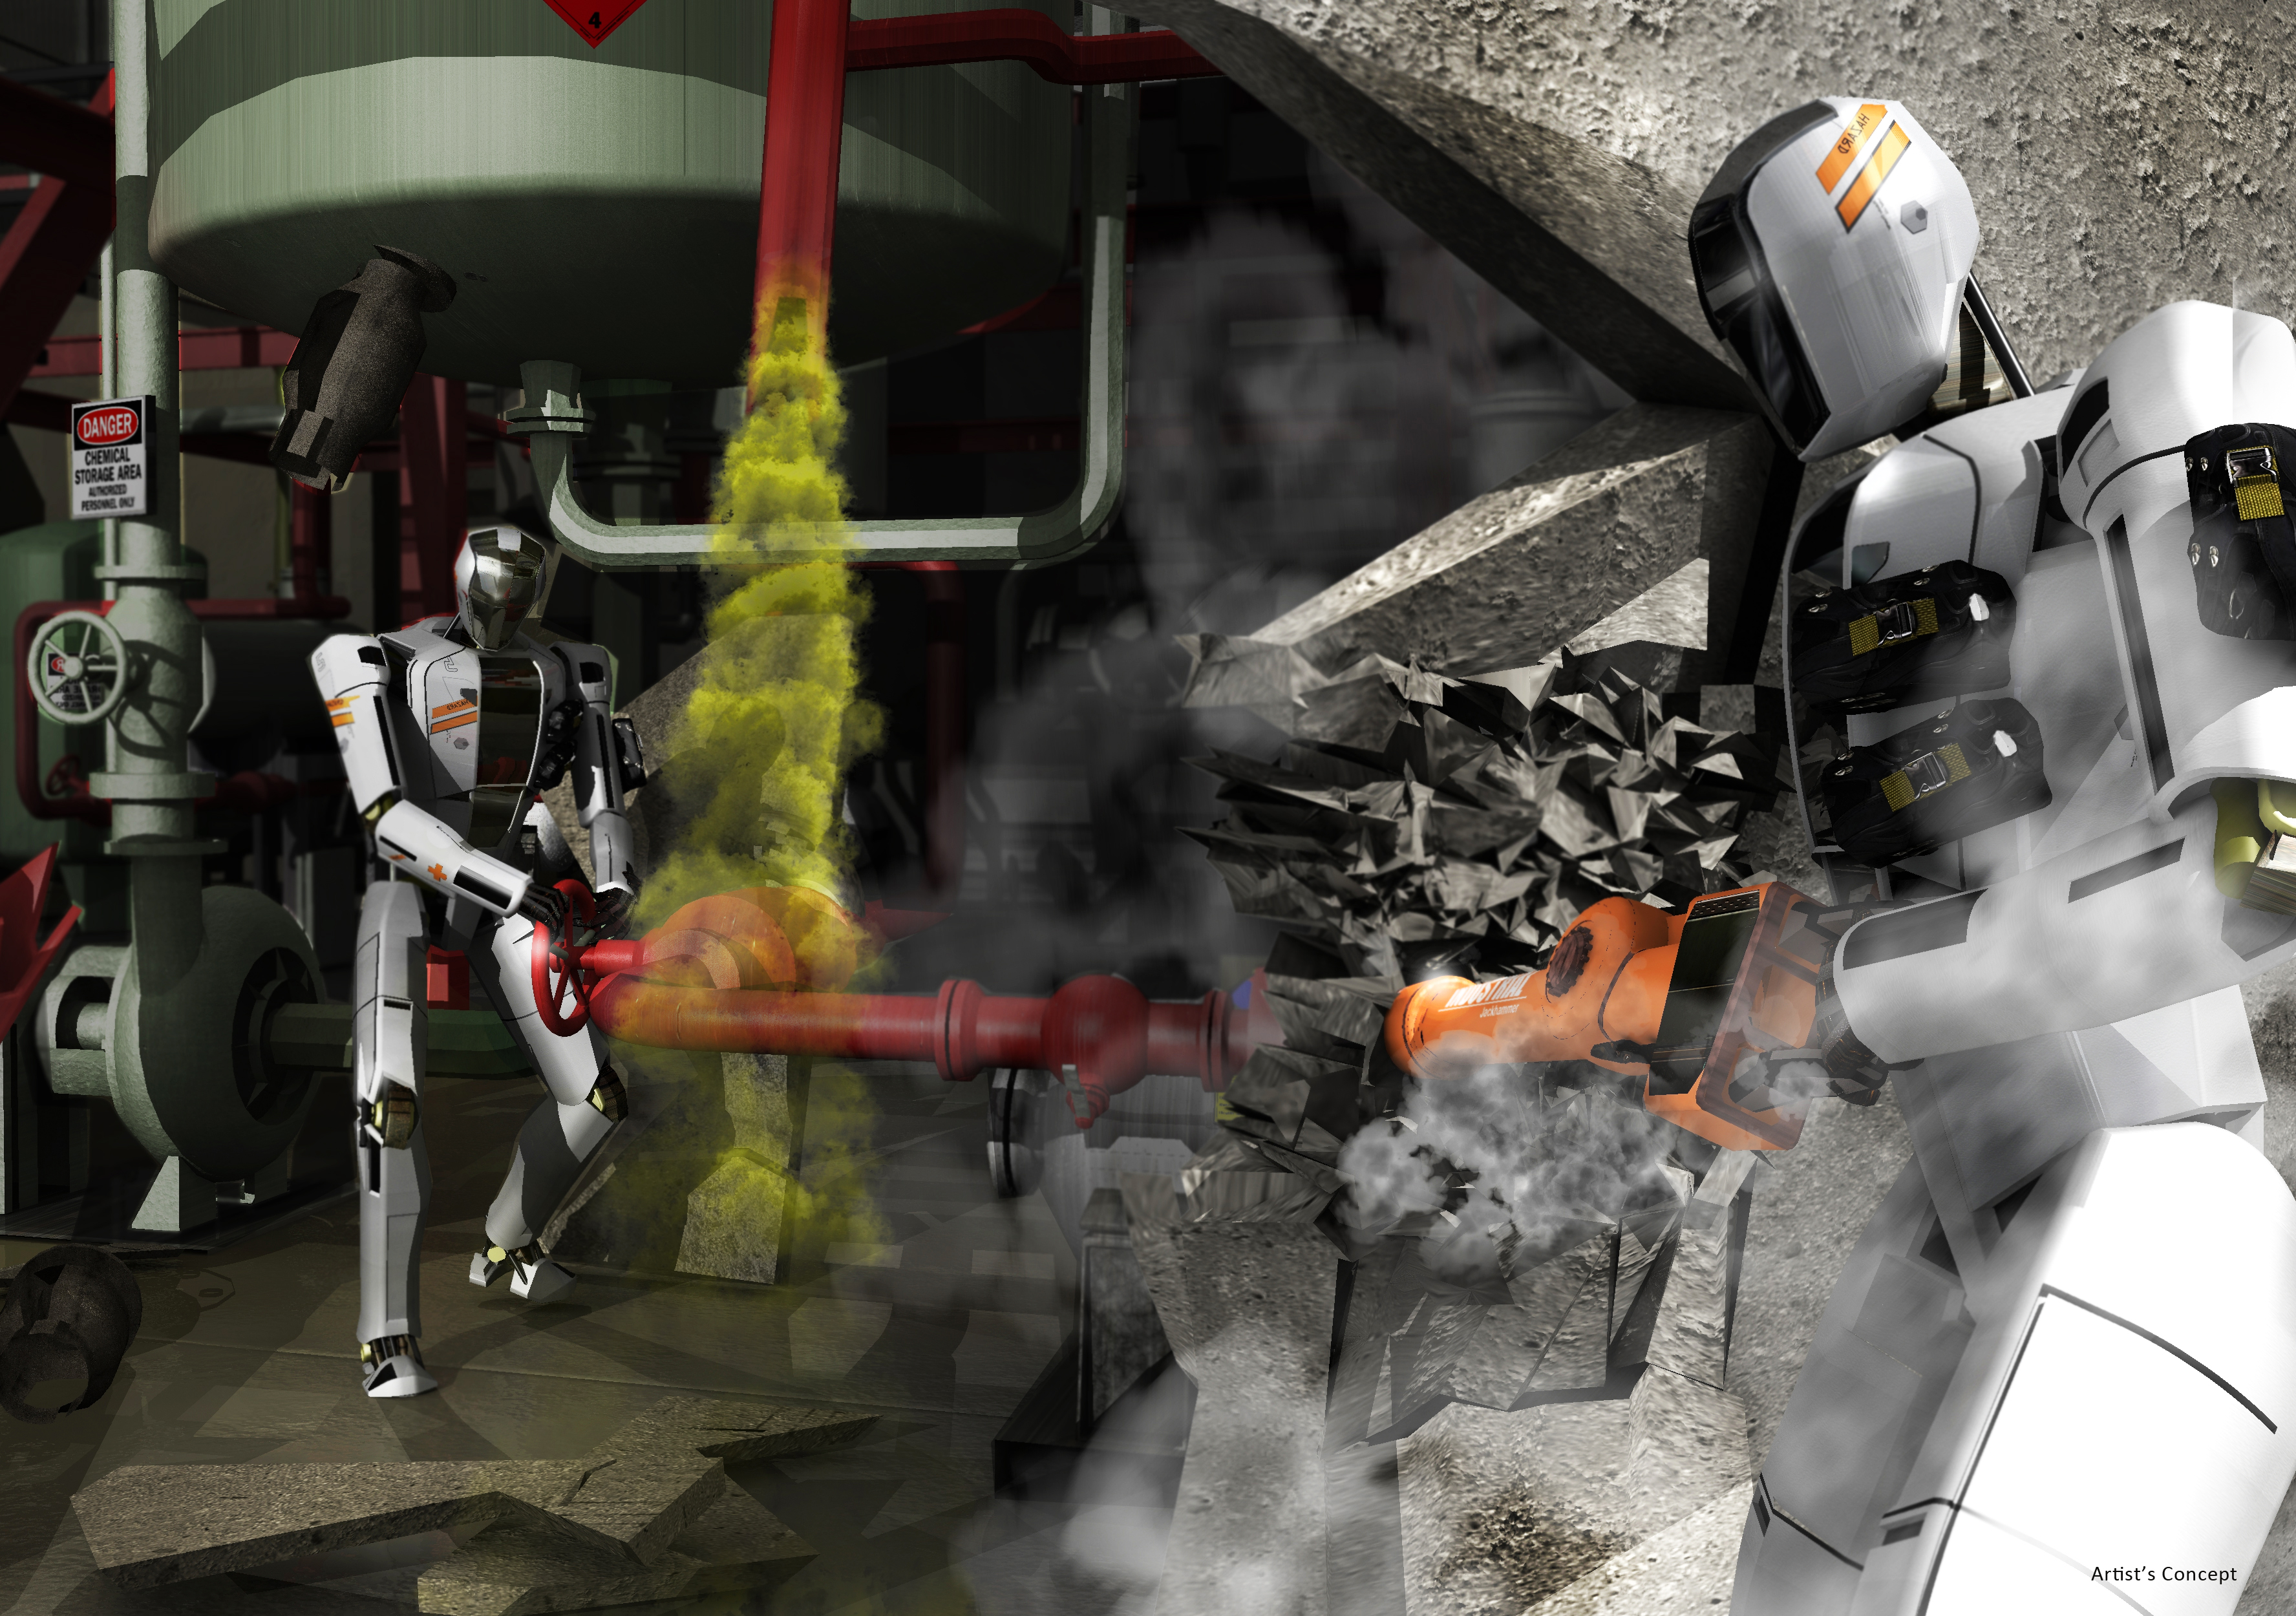
\includegraphics[width=\linewidth]{src/chap5-conclusion/darpa.jpg}
  \end{center}
  \caption{Le défi DARPA pour les robots humanoïdes: les robots
    devront, entre autres, remplacer une vanne et détruire un mur pour
    pouvoir y accéder. \label{fig:darpachallenge}}
\end{figure}


Concernant le travail d'exécution de trajectoire sur robots humanoïdes,
le chemin qui reste à parcourir est clair: pour pouvoir asservir une
trajectoire automatiquement, il faut encore valider la correction des
trajectoires de manipulation, ainsi que l'utilisation d'algorithmes de
vision pour estimer la déformation nécessaire de la trajectoire des
bras. Une fois les tâches de locomotion et de manipulation asservies,
il faudra alors prendre en compte ces contraintes dans la phase de
planification. À l'heure actuelle, le planificateur peut générer un
plan de mouvement, mais il ne prend pas en compte la visibilité des
amers dans la phase de génération de la trajectoire. Il faut
privilégier les chemins assurant une qualité maximale de
l'asservissement. Les contraintes imposées par les systèmes de
localisation variant selon les cas, un dialogue entre l'étage de
planification et l'étage de perception et localisation est nécessaire.
La dernière étape serait alors de ne plus se contraindre à des
transitions temporelles dans le plan, mais également insérer des
événements logiques. Pour ce faire, il sera nécessaire d'insérer dans
l'architecture un superviseur de haut niveau permettant de réaliser la
transition entre les états logiques ainsi que de gérer les retours sur
erreur.


En conclusion, les travaux entrepris durant ces trois ans ont permis
de poser les fondations de l'exécution de trajectoires asservies sur
le robot humanoïde HRP-2, mais il reste encore un important effort à
fournir pour arriver à exécuter des scénarii longs et précis de
manière fiable. Il est fort probable que les années à venir voient
d'importants travaux dans ce sens, le prochain défi proposé par la
DARPA\index{DARPA} \citep{12darpa} étant destiné aux robots humanoïdes
-- voire \autoref{fig:darpachallenge} --. Ces derniers devront
réaliser des mouvements complexes tels que monter une échelle ou bien
encore conduire une petite voiture. Les techniques de fermeture de
boucle comme celle qui a été proposée dans ce manuscrit joueront sans
doute un grand rôle dans la réussite de scénarii de ce type.
